\documentclass{standalone}
\usepackage[usenames,dvipsnames]{xcolor}
\usepackage{tikz}
\usetikzlibrary{arrows.meta}
\usepackage{pgfplots}


\begin{document}

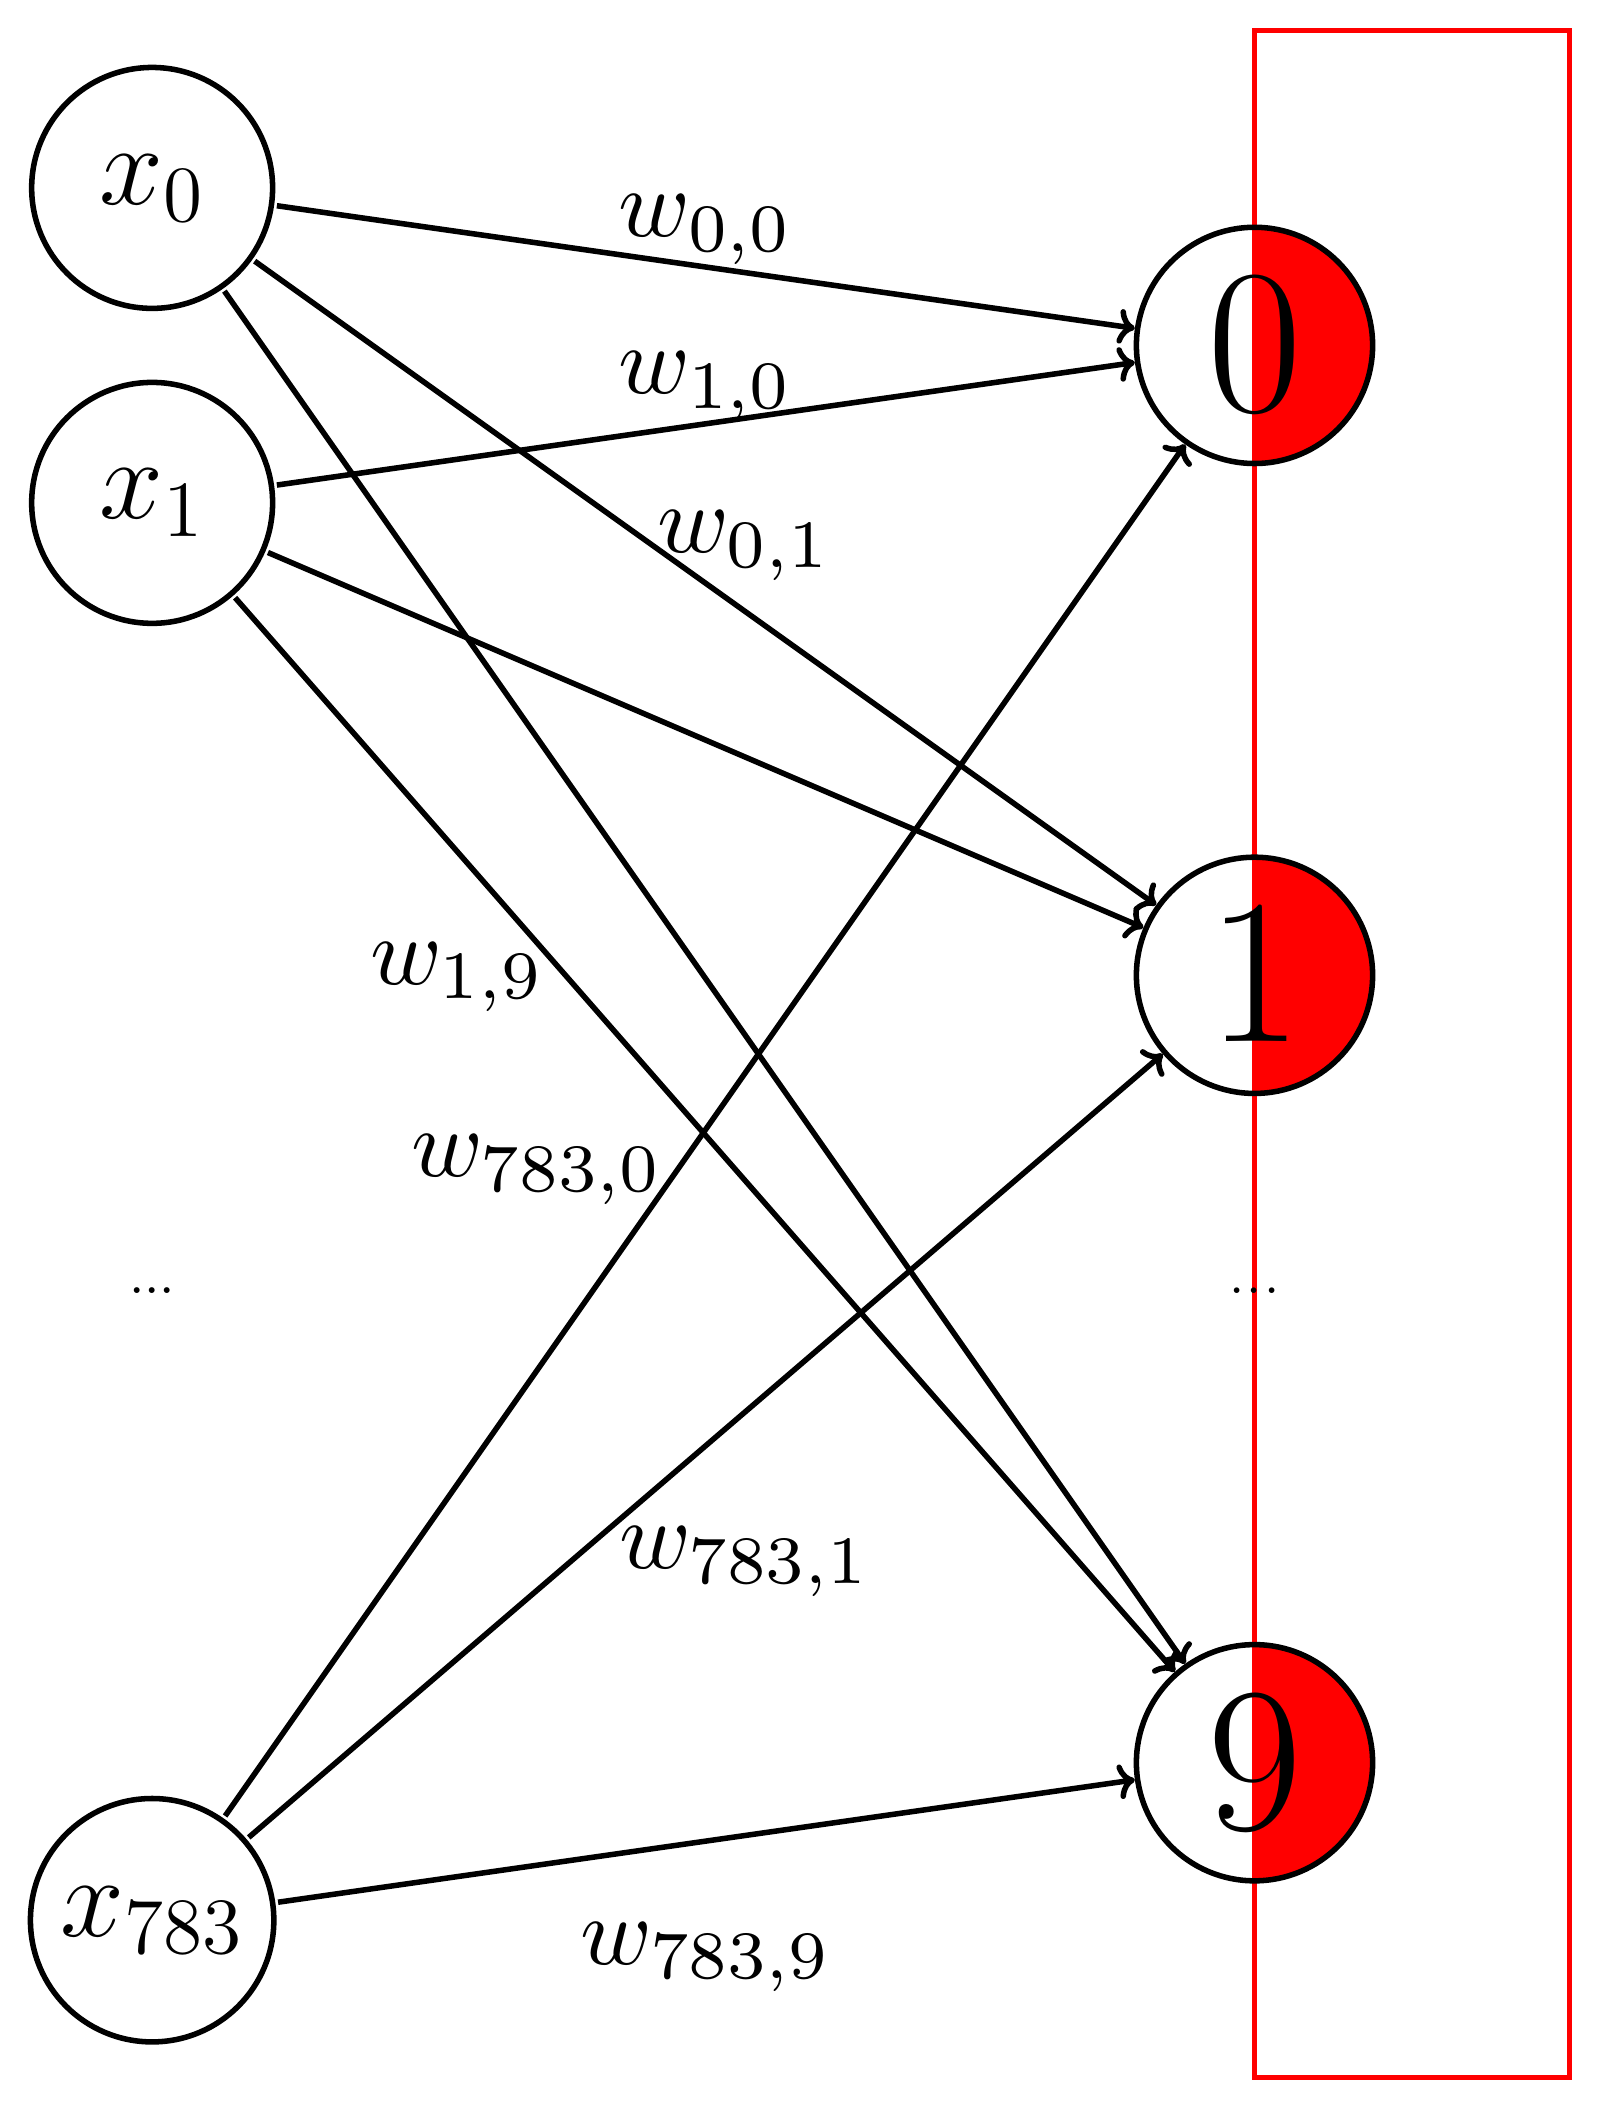
\begin{tikzpicture}

\draw[line width=2, color=red] (7, 14) rectangle (11, -12);

% modify thickness

% input nodes

\node[draw, scale=2, line width=2, circle, minimum size=1.53cm] (x0) at (-7, 12) {\huge $x_0$};
\node[draw, scale=2, line width=2, circle, minimum size=1.53cm] (x1) at (-7, 8) {\huge $x_1$};
\node[scale=2, line width=2, circle, minimum size=1.53cm] (xother) at (-7, -2) {$...$};
\node[draw, scale=2, line width=2, circle, minimum size=1cm] (x783) at (-7, -10) {\huge $x_{783}$};

% right hemisphere of output nodes
\draw[red, fill=red] (7,11.5) arc(90:-90:1.5) -- (7,9.5) -- (7,11.5);
\draw[red, fill=red] (7,3.5) arc(90:-90:1.5) -- (7,1.5) -- (7,3.5);
\draw[red, fill=red] (7,-6.5) arc(90:-90:1.5) -- (7,-8.5) -- (7,-6.5);

% output nodes

\node[draw, line width=2, circle, minimum size=3cm] (y0) at (7, 10) {};
\node[draw, line width=2, circle, minimum size=3cm] (y1) at (7, 2) {};
\node[line width=2, minimum size=3cm] (yother) at (7, -2) {\Huge ...};
\node[draw, line width=2, circle, minimum size=3cm] (y9) at (7, -8) {};

\node[scale=3] (y0_label) at (7,10) {\Huge 0};
\node[scale=3] (y1_label) at (7,2) {\Huge 1};
\node[scale=3] (y9_label) at (7,-8) {\Huge 9};

% bias
%\node[scale=2.5] (b0) at (7, 14) {\Large $b_0$};
%\node[scale=2.5] (b1) at (7, 6) {\Large $b_1$};
%\node[scale=2.5] (b9) at (7, -4) {\Large $b_9$};

% bias to outputs
%\draw [->, line width=2] (b0) edge (y0) (b1) edge (y1) (b9) edge (y9);

% input to output
\draw [->, line width=2] (x0) -- node[above, shift={(0, -0.5)}, scale=3.5] {$w_{0,0}$} (y0); 
\draw [->, line width=2] (x0) -- node[above, shift={(0.5, -0.5)}, scale=3.5] {$w_{0,1}$} (y1); 
\draw [->, line width=2] (x0) -- (y9) ; %node[above, shift={(0, -0.5)}, scale=3.5] {$w_{0,9}$} (y9); 

\draw [->, line width=2] (x1) -- node[above, shift={(0, -0.5)}, scale=3.5] {$w_{1,0}$} (y0); 
\draw [->, line width=2] (x1) -- (y1) ; %node[above, shift={(0, -0.5)}, scale=3.5] {$w_{1,1}$} (y1); 
\draw [->, line width=2] (x1) -- node[left, shift={(-1.5, 2)}, scale=3.5] {$w_{1,9}$} (y9); 

\draw [->, line width=2] (x783) -- node[left, shift={(0, -0.5)}, scale=3.5] {$w_{783,0}$} (y0); 
\draw [->, line width=2] (x783) -- node[below, shift={(0.5, -0.5)}, scale=3.5] {$w_{783,1}$} (y1); 
\draw [->, line width=2] (x783) -- node[below, shift={(0, -0.5)}, scale=3.5] {$w_{783,9}$} (y9); 



%(x1) edge (y0) (x783) edge (y0);
%\draw [->, line width=2] (x0) edge (y1) (x1) edge (y1) (x783) edge (y1);
%\draw [->, line width=2] (x0) edge (y9) (x1) edge (y9) (x783) edge (y9);


\end{tikzpicture}
\end{document}